\chapter{Дополнительная лекция}
\lecture{M + НоД}{12 march}{Набирал Даниил Любаев}
\section{Замощения плитками Ванга}

\begin{figure}[ht]
    \centering
	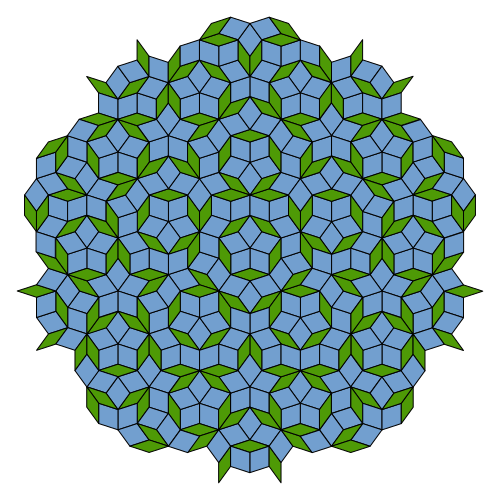
\includegraphics[scale=0.75]{./imgs/Penrose_Tiling.png}
	\caption{Замощение Пенроуза}
\end{figure}
Замещение Пенроуза не периодично, то есть \textit{апериодично}, но покрывает всю плоскость.

Основная наша цель -- доказать, что если нам дан на вход набор 11-и плиток Ванга, то
нельзя выяснить, можно ли ими замостить плоскость (то есть, эта задача неразрешима).

Задача формулируется так -- даются плиточки $ 1 \times 1 $, мы их можем помещать в целочисленные точки плоскости. Каждую из сторон мы можем помечать, например, цветами -- скажем, левую и верхнюю сторону -- красной, правую -- фиолетовой, нижнюю -- желтой. Ставить рядом можно только стороны одинакового цвета.


\begin{defn}[Замощение]
    \selectedFont{Замощение} --- это отображение $ t\colon  \mathbb{Z}^2 \to T $, где $ T $ -- набор плиток.
\end{defn}

\begin{note}
    Самих плиток бесконечно, но количество их типов -- конечно.
\end{note}

\begin{ex}
    Если плитка типа 1 -- справа и сверху синий цвет, а снизу и слева -- красный, а плитка типа 2 -- наоборот, то получится только шахматное замощение.
\end{ex}

\noindent \textbf{Вопрос, который задавал Ванг (1961):} \textit{если дан на вход набор плиток, существует ли алгоритм, проверяющий существование замощения?}

Вопрос решил его студент Berger в 1966 году, доказав неразрешимость.
Мы докажем упрощенный вариант -- замощение \textit{c зерном.}

\begin{thm}
    Задача замощения с зерном (то есть, когда выделенная плитка $ s \in T $ обязана присутствовать в замощении) алгоритмически неразрешима.
\end{thm}
\begin{proof}
    Сведем задачу остановки машины Тьюринга на пустой ленте.

    Дана $ M = (Q, \Sigma, \Gamma, , \delta, q_0, f)$, где $ f $ -- конечно. Пробел обозначаем за $B$ (blank).

    Строим $T$:
    \begin{enumerate}
        \item Плитки инициализации.
\begin{figure}[ht]
    \centering
    \incfig{init-tails}
	\caption{Плитки инициализации}
    \label{fig:init-tails}
\end{figure}
        \item  Плитки алфавита
\begin{figure}[ht]
    \centering
    \incfig{alphabet-tails}
    \caption{Плитки алфавита}
    \label{fig:alphabet-tails}
\end{figure}
        \item Плитки переходов. 
			Если есть команда $ \delta(q, a) = (p, b, t) $, то сопоставляем
			ей плитку $ (1)$.

			Если команда $ \delta(q, a) = (p, b, \rightarrow) $, то плитка  $ (2)$.
\begin{figure}[ht]
    \centering
    \incfig{delta-tails}
    \caption{Плитки перехода}
    \label{fig:delta-tails}
\end{figure}
        \item Плитки склеивания.
\begin{figure}[h!]
    \centering
    \incfig{bonding-tails}
    \caption{Плитки склеивания и пустая плитка}
    \label{fig:bonding-tails}
\end{figure}
        \item Пустая плитка, чтобы заполнить низ. 
    \end{enumerate}

    Посмотрим теперь, как плитки устроены и как мы будем делать сведение.

    Начинаем с зерна (потому что оно должно присутствовать). Что мы можем к ней приписать справа?
    Только одну из плиток инициализации (какую, видно из картинки). Слева -- аналогично.

    Какую можем вниз? Только плитку типа 5.

    Какую можем сделать при шаге машины Тьюринга? Выглядит это примерно так:
\begin{figure}[ht]
    \centering
    \incfig{step-mt}
    \label{fig:step-mt}
\end{figure}

    Все остальное -- плитки склеивания, вариантов нет.

\begin{figure}[ht]
    \centering
    \incfig{imitaion-mt}
    \caption{Имитация МТ}
    \label{fig:imitaion-mt}
\end{figure}

    Продолжается это бесконечно, потому что если машина остановится, то это будет конечное число
    шагов, и мы не сможем прилепить плитку (потому что переход будет не определен).

    Метки бесконечных строк составляют конфигурацию машины Тьюринга. Замощения существуют тогда и только тогда, когда машина Тьюринга не останавливается. Получается, если бы мы умели решать задачу замощения, то мы бы могли сказать, остановится ли машина Тьюринга.
\end{proof}

\begin{lm}
    Если для любого $ n $ существует замощение квадрата $ n \times n $, то существует замощение всей плоскости.
\end{lm}
\begin{proof}
    Аналог леммы Кенига о том, что в бесконечном дереве существует бесконечная ветвь. Или так: любая плитка встречается бесконечно много раз. Смотрим ее возмозные продолжения до квадратика $ 2 \times 2 $. Какой-то из этих вариантов встречается бесконечно много раз -- выберем его. Смотрим ее продолжения до квадратика $ 3 \times 3 $, и т.д.
\end{proof}

\begin{cor}
    Неразрешимость в купе с леммой дает существование апериодических замощений, то есть наборов плиток, для которых существуют только непериодические замощения.
\end{cor}
\begin{proof}
    Иначе можем красить увеличивающиеся квадраты $ n \times n $, либо придем к противоречию,
    либо увидим период.
\end{proof}

\begin{lm}
    Если для данного набора плиток существует замощение, периодическое в одном направлении, то существует и замощение, периодическое в двух направлениях.
\end{lm}
\begin{proof}
    Пусть $(a, b)$ -- вектор периодичности (то есть, если сдвигаем плитку на вектор $ (a, b) $ то там та же плитка).

    Рассмотрим кусочки такого размера *картинка*

    Квадратов бесконечно, способов замостить конечно, поэтому какой-то встретится два раза. При этом цвета снизу такие же,
    как и сверху (потому что период).
    Значит красным квадратом мы можем замостить все.
\end{proof}

\begin{figure}[ht]
    \centering
    \incfig{kari-tiles}
    \caption{Плитки Кари}
    \label{fig:kari-tiles}
\end{figure}
\begin{thm}[про 14 плиток]
    Плитками с картинки можно замостить плоскость, но только апериодическим способом\footnote{Подчеркнутые и не подчеркнутые цифры -- разные.}.
\end{thm}
\begin{proof}
    Надо доказать, что замощение существует, и что не существует периодического.
    *тут было очень много слов и я не успевал, нужно написать эту теорему с видео*
\end{proof}


